\documentclass[10pt]{article}
\usepackage[utf8]{inputenc}
\usepackage{geometry}
\usepackage[T1]{fontenc}
\usepackage{amsfonts}
\usepackage{graphicx}
\usepackage{float}
\usepackage{hyperref}
\usepackage[sorting=none]{biblatex}
\usepackage{fancyhdr}
\usepackage{multicol}
\usepackage{utopia}
\addbibresource{ref.bib}
\fontfamily{put}\selectfont
\setlength{\columnsep}{40pt}
\setlength{\voffset}{0.5cm}
\setlength{\headsep}{40pt}
\geometry{legalpaper, portrait, margin=2.3cm}

\bibliography{ref.bib}


% Title page
\title{Lab Project:\\ \textbf{Hot n' Cold Rubidium}\\\Large{ Under Supervision of Dr. Pablo Solano Palma \\ 2024}}
\author{Amaru Moya y basados \\ Universidad de Concepción\\ Faculty of Physical and Mathematical Sciences, Physics Department}
% \date{\today}

% Header and footer
\pagestyle{fancy}
\fancyhead[C]{
\includegraphics[width=0.05\textwidth]{img/escudo.png}}
\fancyhead[L]{\textbf{Lab Project}\\ Universidad de Concepción}
\fancyhead[R]{\textbf{Amaru Moya R.}\\ amarumoya@udec.cl}
\fancyfoot{}
\begin{document}

\maketitle
\thispagestyle{fancy}

\begin{figure}[h]
    \centering
    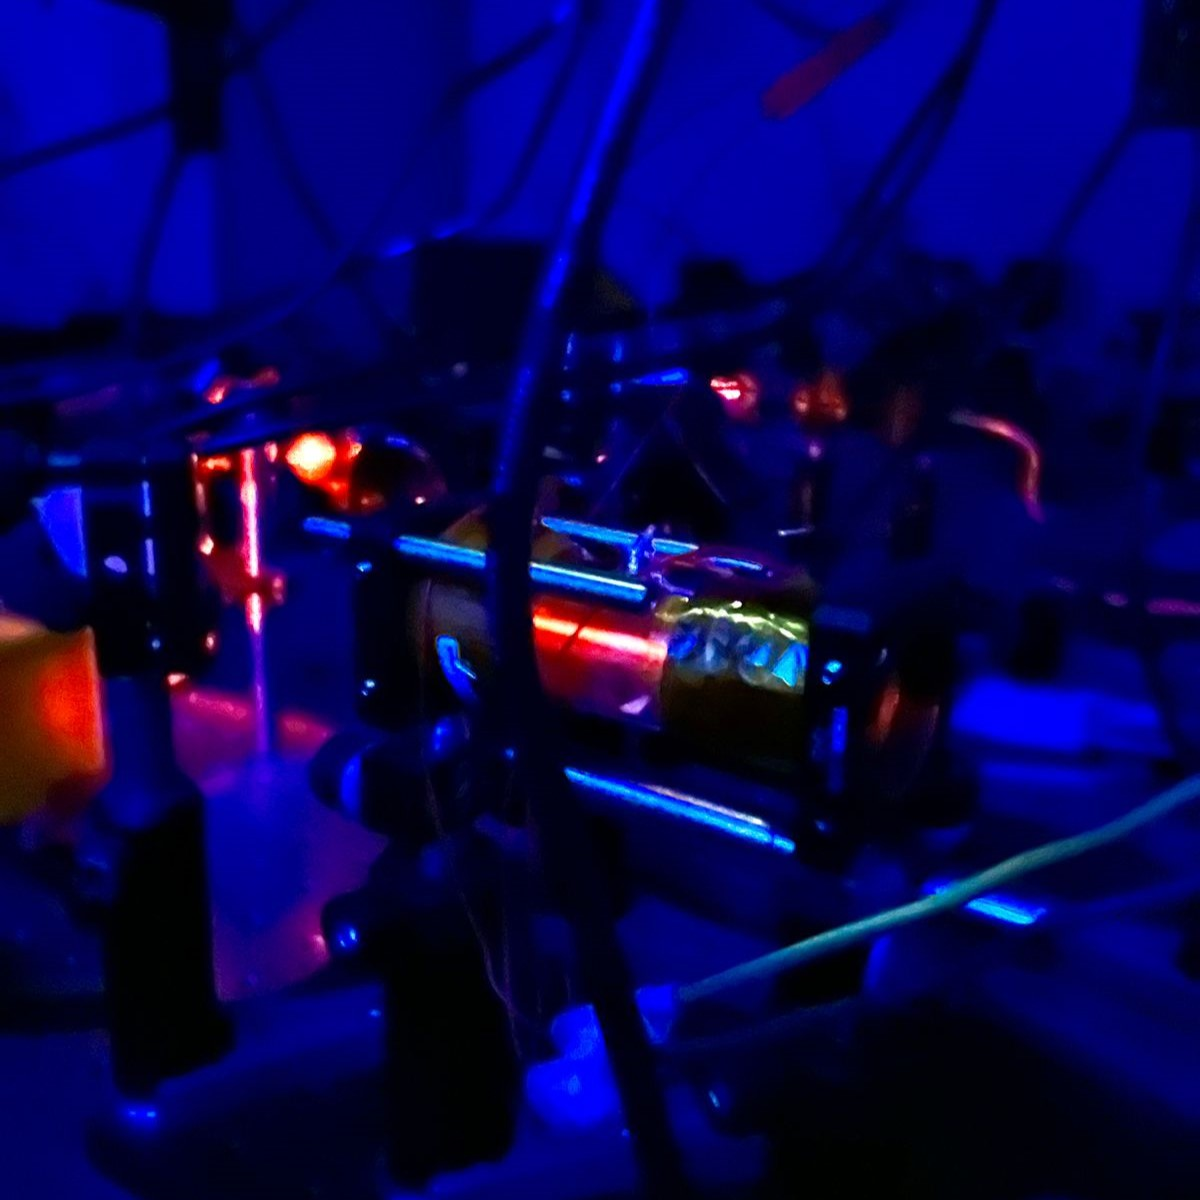
\includegraphics[width=.5\linewidth]{img/resonancia.jpeg}
    \caption{sayans! }
    \label{fig:portada}
\end{figure}

\clearpage
% \tableofcontents
% \thispagestyle{fancy}

% \clearpage
% Begin page numbers
\fancyfoot[C]{\thepage}
\pagenumbering{arabic}
% \begin{multicols}{2}

% pq es interesante, como contribuye con el entendimiento de la naturaleza del ser humano
% estado del arte/ grupos que estudien tematicas similares?
% que evidencia hay que este proyecto pueda resolver el problema planteado?
% compatibilidad en los recursos, tiempos y problemas


% estado del arte y fundamentos,% revision de conceptos tecnicos

% preguntas hipotesis y objetivos, potencial impacto

% marco metodologico, objetivos

\section*{Summary}
\addcontentsline{toc}{section}{Introduction} % For the contents page

% Describa los principales temas que se abordarán en el proyecto: objetivos, metodología y resultados esperados. La extensión máxima de esta sección es de 1 página (utilizar formato tamaño carta, fuente Verdana tamaño 10 o similar).


\noindent The main objective of this project is to study and manipulate the index of refraction of a Rubidium vapour through the interaction with laser light of two different wavelengths. Using a theoretical, numerical and experimental approach, we aim to understand and characterize the Rubidium vapour and the effects of light interacting with this system. The project will be divided into three main stages: theoretical study, numerical simulations, and experimental validation. The theoretical study will focus on the fundamentals of atomic quantum optics, with emphasis on the interaction between light and matter. The numerical simulations will be used to model the interaction between light and Rubidium vapour, and to predict the behaviour of the system under different conditions. Finally, the experimental validation will involve the construction of an experimental setup to measure the index of refraction of the Rubidium vapour and compare the results with the theoretical and numerical predictions. The expected results of this project include a better understanding of the interaction between light and matter, and the development of new techniques for manipulating the index of refraction of Rubidium vapour. This research has the potential to have a significant impact on the field of quantum optics and quantum information processing, and to open up new possibilities for the development of quantum technologies.


\newpage
\section*{Rubidium}
Rubidium is composed naturally of two stable isotopes, $^{85}$Rb and $^{87}$Rb.
\subsection*{Atomic Structure}
% Rb Structure, Dlines, 

\begin{figure*}[h]
    \centering
    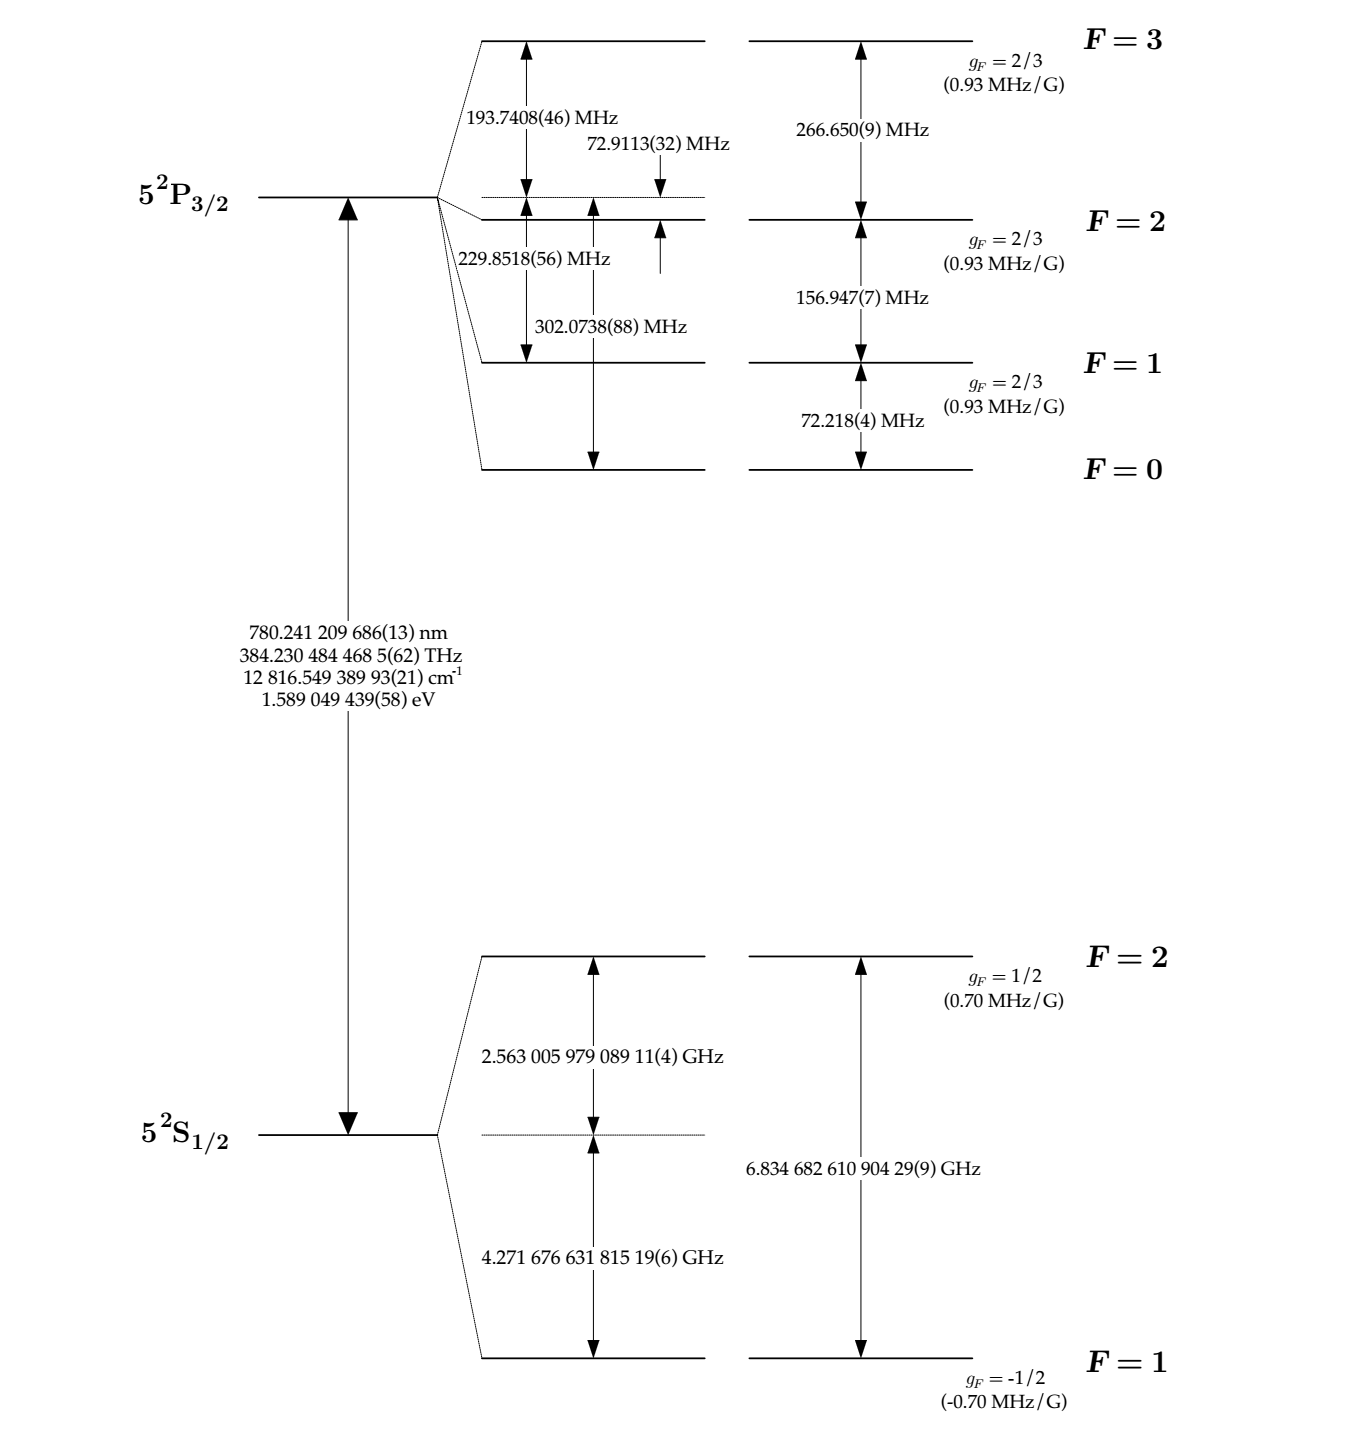
\includegraphics[width=0.9\textwidth]{img/rb87D2.png}
    \caption{$^87$Rb $D2$ transition hyperfine structure, with frequency splittings between the hyperfine energy levels.The approximate Landé
    $g_F$-factors for each level are also given, with the corresponding Zeeman splittings between adjacent magnetic sublevels. (Steck, 2001) }
    \label{fig:image1}
\end{figure*}


\section*{Laser 1}

\begin{figure}[h]
    \centering
    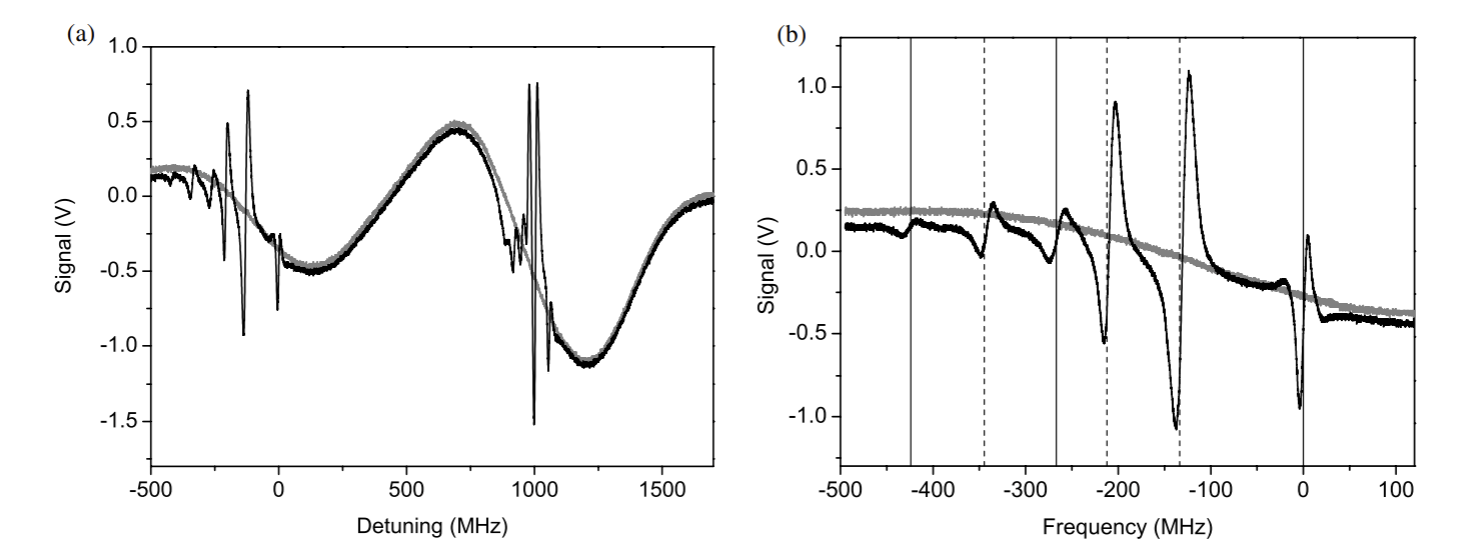
\includegraphics[width=0.9\textwidth]{img/brrr.PNG}
    \caption{(a) Typical sub-Doppler DAVLL spectra recorded for the F = 2 → F line in 87Rb and F = 3 → F 85Rb (black line). The
    sub-Doppler features are superimposed on the conventional DAVLL signal (grey line) obtained by blocking the pump beam. (b) A
    zoomed-in section of (a) showing the sub-Doppler DAVLL signal for the F = 2 → F transitions of 87Rb. Vertical lines indicate the
    expected line centres of the three transitions (solid lines) and three crossovers (dashed lines). Small discrepancies in the location of spectral
    features relative to the line centres arise from the slightly nonlinear laser scan. Spectra were taken at a magnetic field of 9.5 G, a pumppower of 154 µW and a probe power of 20 µW. doi:10.1088/0953-4075/41/8/085401}
    \label{fig:curvas}
\end{figure}


\begin{figure*}[h]
    \centering
    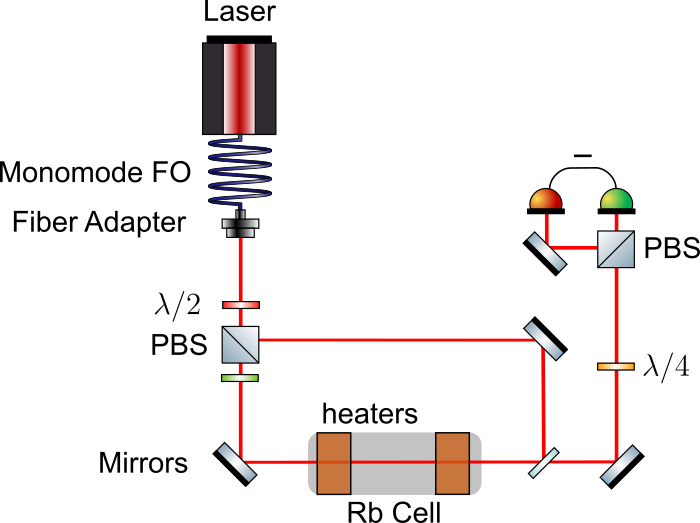
\includegraphics[width=0.5\textwidth]{img/rect5909.png}
    \caption{Set up for Laser 1. Dicroich atomic vapor laser lock (DAVLL) system.}
    \label{fig:laser1}
\end{figure*}

\begin{enumerate}
    \item Osciloscope
    \item Signal Generator
    \item TEC: Temperature Control
    \item Control of Control : Lockbox
    \item Laser Control : Negative Current Control
    \item Current Control %(Coil de la válvula)
    \item Rubidium Heater for Glass Cell
\end{enumerate}

\section*{Laser 2}

\section*{Laser 3}


\section*{Bragg Reflections in Rubidium Vapours}

\begin{figure}
    \centering
    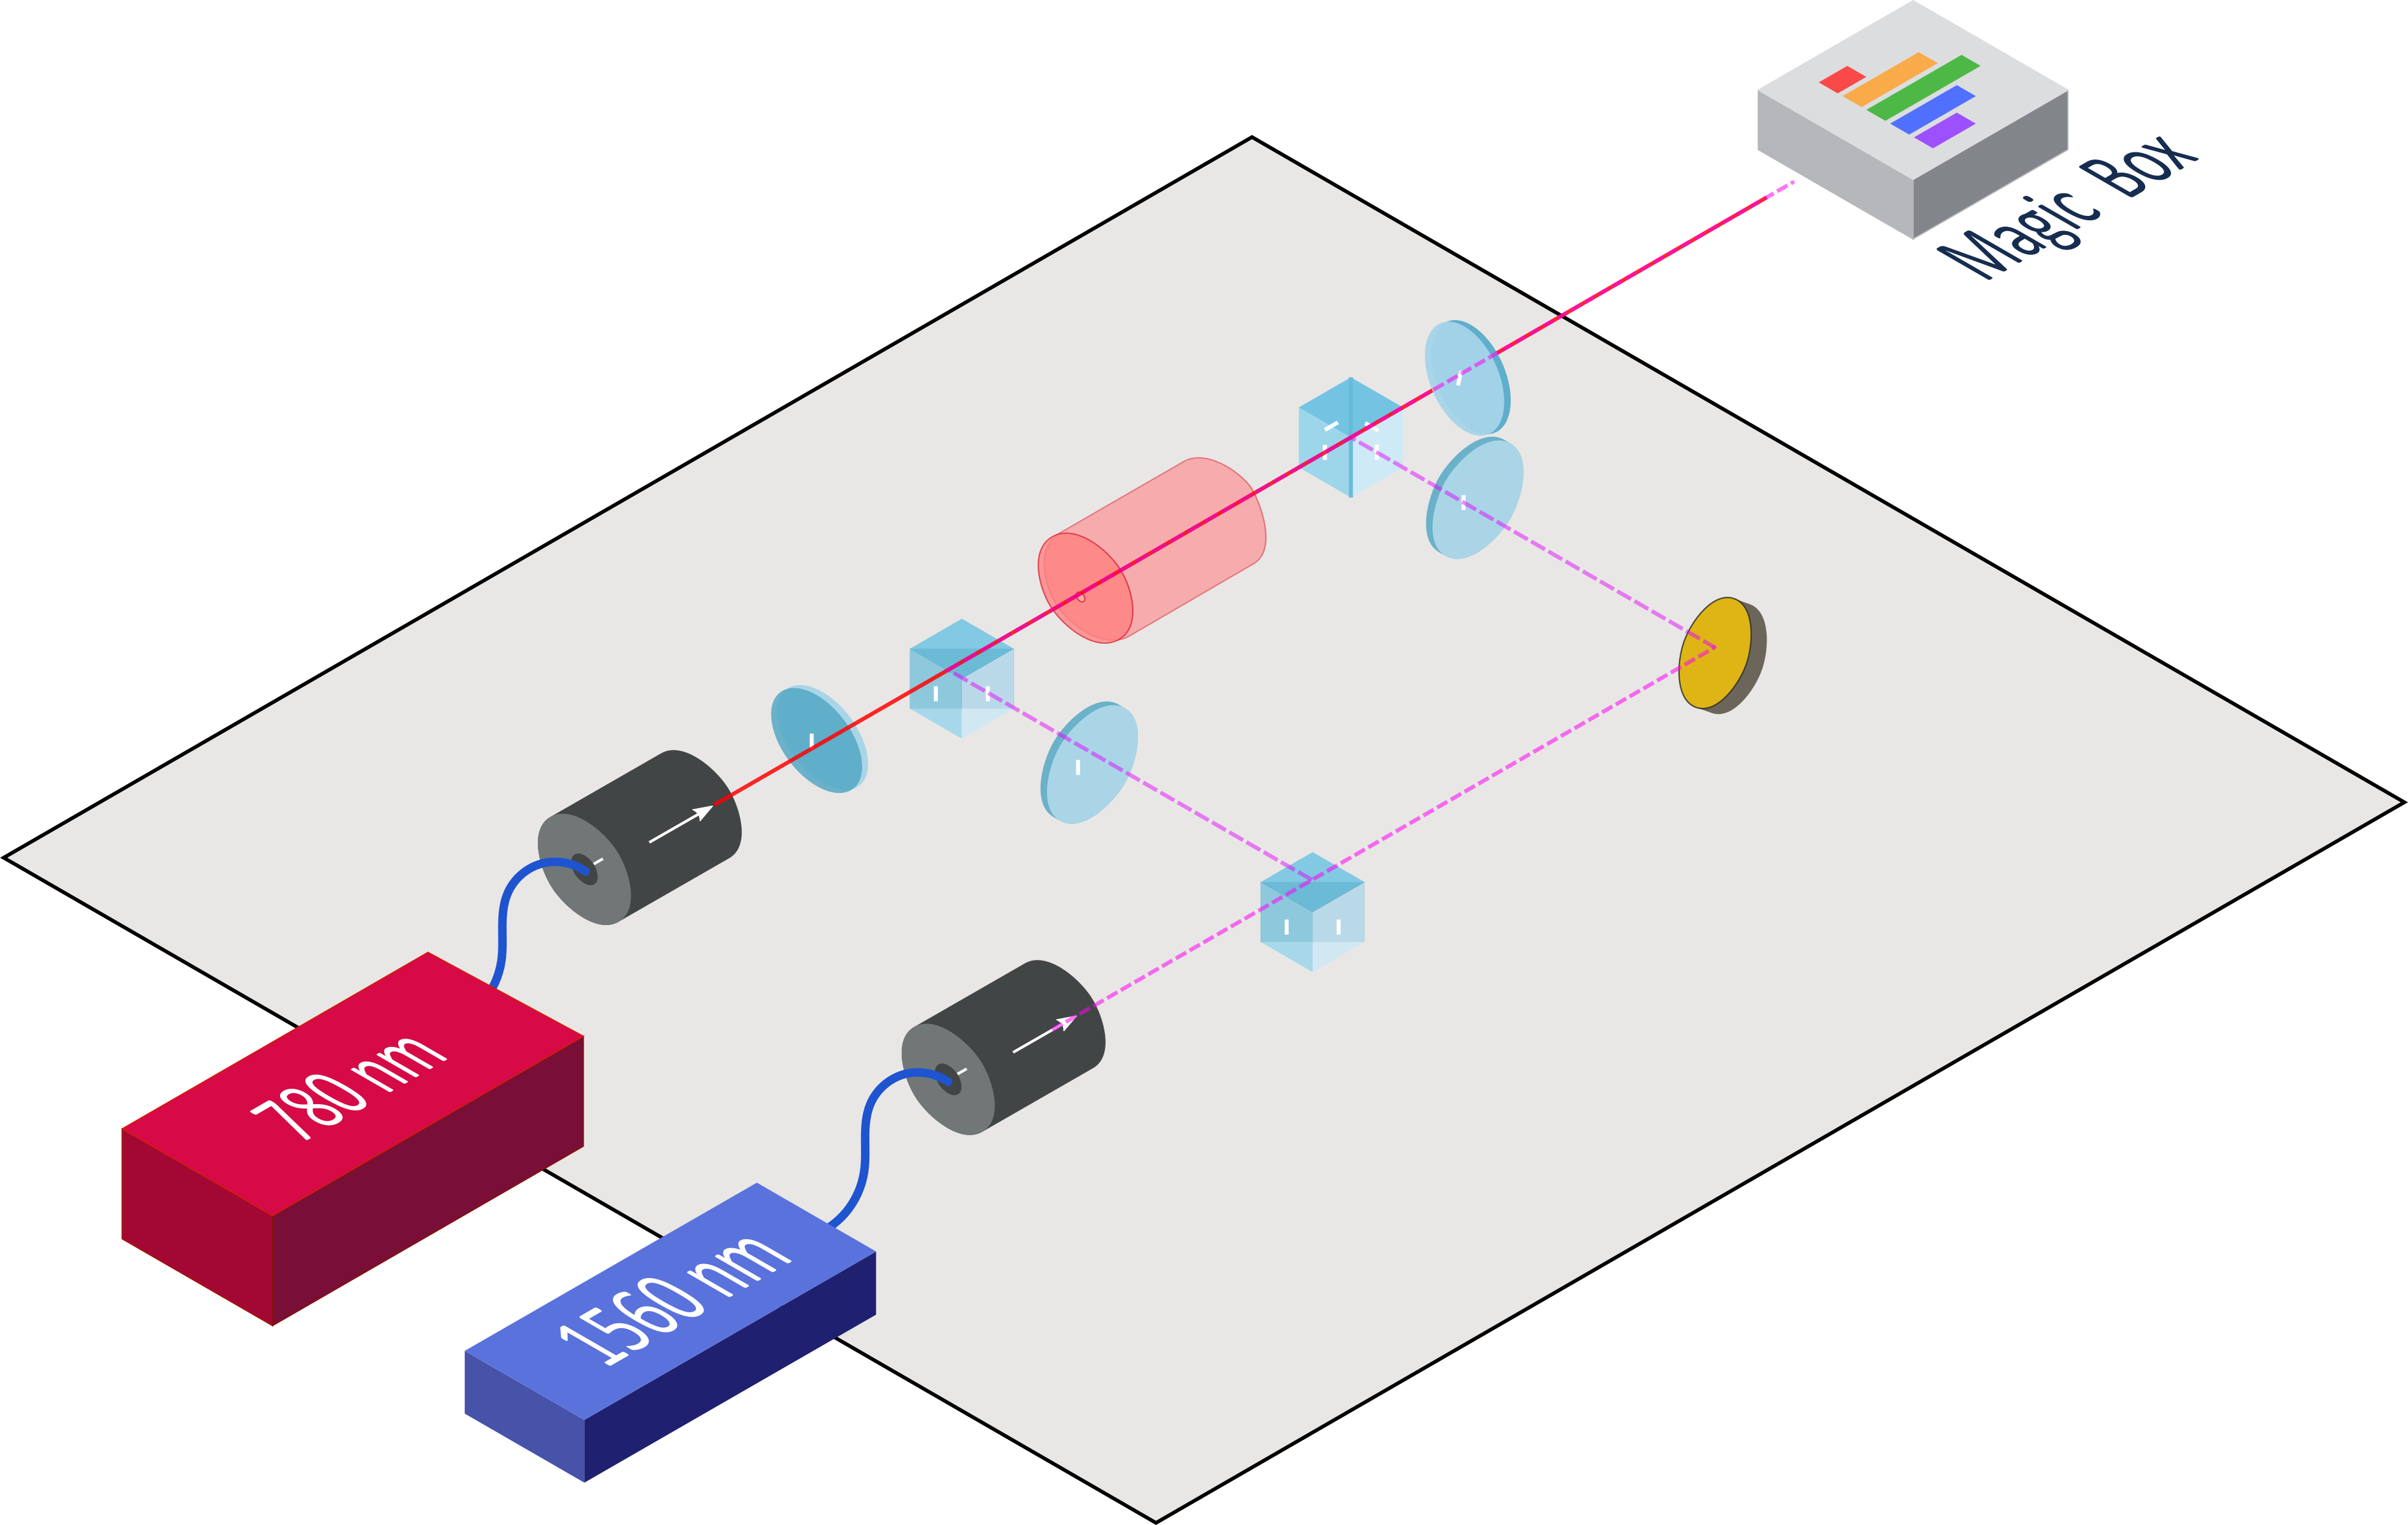
\includegraphics[width=0.6\textwidth]{img/path16176.png}
    \caption{Set up for the experiment of the bragg Vapours.}
    \label{fig:braggref1}
\end{figure}





\subsection*{Experimental Set Up}
\textbf{Rubidium Borosilicate Reference Cell, Ø25.4 mm x 71.8 mm } :
Since each fill material is associated with a unique absorption spectrum that serves as its fingerprint, the contents of a reference cell can be determined via a linear absorption measurement (as depicted by the simplified schematic above). By scanning a tunable diode laser over a wavelength range and detecting light absorption (A) with a photodetector, a series of peaks will be recorded, which is characteristic of the vapor inside the cell.
All of the cells offered here are baked and evacuated to 10-8 Torr prior to filling in order to remove contaminants. Additionally, each cell is helium leak checked to ensure the longevity of the vapor cell. The vapor pressure of the alkali metal will cause it to migrate throughout the cell and condense at the coolest area. Heating the windows of the cell rather than the cell body will help ensure the windows stay warmer and thus that the alkali will collect elsewhere. If obstruction of the optics becomes an issue, apply cooling to an area on the cell body, such as near the fill stem, and heat the windows in an alternating fashion to drive the metal from the window surfaces and collect it at the cool spot. The metal may eventually move back to the windows depending on how the cell is heated.
The rubidium reference cell (GC19075-RB) is sold with the natural isotope ratio of Rb, which is $72.15\% \, ^{85}$Rb and $27.85\% \, ^{87}$Rb  \\
%GC25075-RB	
\textbf{SM1FCA - FC/APC Fiber Adapter Plate with External SM1 (1.035"-40) Threads, Wide Key (2.2 mm)}

\subsection*{Doppler broadened absorption in a vapor cell}
The rubidium atoms in the vapor cell are moving according to the Maxwell-Boltzmann velocity distribution at a temperature of around 400 K. The Doppler broadened lines have line widths of several 100 MHz. This is because even if we detune the probe light by several 100 MHz from the resonance frequency for an atom at rest, there are still atoms within the vapor cell that are moving at the right velocity relative to the wavevector of the light so that they see the light as being exactly on resonance in their center-of-mass frame. Those atoms absorb light from the incident beam, and thereby attenuate the light beam passing through the vapor cell.

\section*{Bragg Reflections in Cold Rubidium}




\subsection*{Experimental Set Up}


\subsection*{MOT - Atom Trapping}
e. Invented at MIT and first demonstrated at Bell Labs [4], it combines the abilities of both cooling and also trapping atoms, limiting both their momenta and their positions, while remaining experimentally simple to implement and to integrate with other experimental needs. Using MOTs and other laser cooling methods, a wide variety of ultracold atomic and molecular gases are produced routinely in labs around the world and applied to a range of scientific pursuits, e.g. matter-wave interferometry with coherent atomic beams, condensed-matter like systems created from quantum-degenerate gases, and novel atomic clocks and other modes of precision measurement.

\begin{enumerate}
    \item Scattering Rate
    \item Radiation Pressure
    \item Doppler Shift
    \item Doppler Cooling
    \item Capture Velocity
    \item Doppler Temperature Limit and Doppler Molasses
    \item Effects of the Zeeman shift on light scattering
    \item Sub-Doppler Cooling
    \item 
\end{enumerate}

\newpage
\section*{References}

% Incluya en esta sección, el listado de referencias bibliográficas completas citadas en la sección Formulación de la Propuesta. Extensión: 2 páginas (utilizar formato tamaño carta, fuente Verdana tamaño 10 o similar).

% por lo menos 20 que tengo que manejar bien


\end{document}
